
%% Include weights of evidence example! Can make reference to the white paper.
\chapter{Credit Case Study}

\section{Problem Statement}
Companies which operate in the credit environment want to see returns on their investments. Before a loan is granted to a prospective client the appropriate risk analysis needs to be performed. In many instances this is a manual process where a credit employee has to assess a clients credit portfolio and ascertain if they are eligible for a loan and if so, on what terms. As most manual processes it can be slow and prone to human-error. By adopting machine-learning we are able to eliminate the human risk factor and significantly increase the speed. Linear modelling techniques such as \emph{Logistic Regression} are the preferred choice due to them being inherently interpretable. Interpretability is a strict requirement due to the need to understand why the model is making the decisions that it does. Linear models are however very limited in what they can do and by using Neural Networks or other nonlinear models we may be able to significantly increase our accuracy at identifying risk, however such techniques are generally seen as a \emph{black-box}. In this section we use SHAP in order to gain some interpretability into credit risk Neural Networks so that they could be considered as possible solutions.

\section{Our Data set} Up until this point we have used our tools on \emph{toy} examples where the data has been engineered to work well with machine-learning. In this section we will be using a proprietary synthetic credit dataset which has been provided to us by \emph{Praelexis} which aims to simulate actual features used by credit companies to calculate potential client risk. Our dataset consists of a total of $200000$ client samples where $28768$ defaulted on their loan and the remaining $171232$ did not. As we can see we have a heavy class imbalance in our data with a ratio of roughly $85:15$. In practice this ratio of imbalance can be a lot higher \cite{doi:10.1142/9789812813312_0009}. The trained model may be skewed to more likely predict the most present class. How we solve this issue is discussed in section \ref{sec-class-imbalance}.

\section{Aim}
 Our aim is see if we can provide enough interpretability into a credit Neural Network so that it may be considered a possible alternative to linear models by credit companies looking to adopt machine-learning. In order to achieve this we train a \emph{Logistic Regression} model which is inherently interpretable and a generic feedfoward Neural Network and compare their interpretability. The goal of these models is to predict a probability that a client will default on a loan given their input features. As we have seen in the \emph{Evaluation} section, SHAP is superior to LIME in every way but speed and therefore we shall use SHAP as our preferred tool for interpretation.
 
\section{Weights of evidence}
 The weights-of-evidence (WOE) transformation \cite{Siddiqi2005CreditRS} is a nonlinear transformation of the original variables. It is used measure the strength of each attribute at separating good and bad loans. It can be seen as the measure of the difference in the proportioning of good and bad within each attribute (i.e., the odds of a person of that attribute being good or bad) \cite{Siddiqi2005CreditRS}.  Continuous variables are first converted to categorical variables through a process called \emph{binning}. Using the information from our training data we calculate the WOE value for each bin. Each client is either considered to be good (0) or bad (1).
 The WOE can be calculated as,
  \begin{equation}
     \mbox{WOE} = \left[ \ln{\left(\frac{\mbox{Distr Good}}{\mbox{Distr Bad}}\right)} \right] 
     \label{eq:woe}
 \end{equation}
We can see an example of creating WOE bins for a variable  in Figure \ref{table:woe}. The \emph{boundaries} are the bin ranges and can either be manually or automatically chosen. The \emph{Count good} and \emph{Count bad} is extracted from the training dataset and by using (\ref{eq:woe}) we are able calculate the WOE value for each bin. 
 \subsection{Benefits of WOE}
 \begin{itemize}
     \item Missing values are separated into their own bins and is therefore easier to handle.
     \item Provides a linear relationship with log odds.
     \item It can treat outliers. Extreme values which fall outside the average range are given their own bin.
     \item We are able to determine the stability of our model by comparing the WOE values of our training and unseen data.
     \item Converts continuous variables into categorical variables so that there is no distinction between the 2.
 \end{itemize}
 For our dataset we have chosen to use \emph{automatic binning} because we want our preprocessing steps to be as automated as possible. This is to prevent our domain knowledge from affecting the produced explanations.
 

 
 \begin{table}[h!]
 \scriptsize
\begin{center}
\shadowbox{\begin{minipage}[t]{0.95\textwidth}%
    \begin{tabular}{cccccccc}
       & Bin  &  Boundaries & Count good & Fraction good & Count bad & Fraction bad & WoE\\
       \hline\\
       & $1$ & $(-\infty,1]$ & $1760$ & $0.0973$ & $798$ & $0.2033$ & $-0.37$ \\
       & $2$ & $(1,2]$ & $5238$ & $0.2896$ & $1 223$ & $0.3116$ & $-0.07$ \\
       & $3$ & $(2,3]$ & $7881$ & $0.4357$ & $1 034$ & $0.2634$ &  $\phantom{-}0.50$ \\
       & $4$ & $(3,\infty)$ & $3210$ & $0.1775$ & $870$ & $0.2217$ & $-0.22$ \\
        \hline
    Total & &  & $18 089$ & $1.0$ & $3 925$ & $1.0$ & 
    \end{tabular}
    \end{minipage}}
\par\end{center}
\caption{WOE example}\label{table:woe}
\end{table}
 



\section{Metrics}
Before we discuss our models architecture we introduce the metrics with which we use to measure the performance of our model. Firstly we introduce some terminology used within the metrics definitions. To provide some context, suppose we have a model that predicts whether an insurance claim made by a client is fraudulent or not. Fraudsters which have been correctly identified by our model are referred to as \emph{True Positives (TP)}, where as regular clients which are incorrectly identified as fraudsters are referred to as \emph{False Positives (FP)}. Regular Clients which are correctly identified are referred to as \emph{True Negatives (TN)}, where as fraudsters which are incorrectly identified as regular clients are referred to as \emph{False Negatives (FN)}.
\subsection{Accuracy}
 In most examples the common metric that is used to measure how well a model performs is the \emph{accuracy} measure, however it does not work as well if our dataset has a class imbalance. Suppose in our previous example of identifying fraudulent claims that our training dataset consisted of 95\% legitimate claims and 5\% fraudulent claims. If we engineer our model to simply predict every claim to be legitimate then we will achieve a 95\% accuracy, however our model would never be able to identify fraudulent claims and therefore does not solve our problem. Although a high accuracy does not necessarily mean a model is performing well, a low accuracy can be indicative of a poor performing model and therefore has relevance. Using our previously defined terms we can define accuracy as,
\begin{equation}
    \mbox{Accuracy} = \frac{TN + TP}{FN + FP + TN + TP}
\end{equation}
\subsection{Precision}
An important metric is called \emph{precision} which is the proportion of positive identifications that were actually correct. In our previous example of identifying fraudulent claims, precision would be the percentage of \emph{actual} fraudsters in the group of people that our model has predicted to be fraudsters. Therefore using this measure we are able to determine the ratio of how many of our regular clients we have falsely predicted to be a fraudster. We define precision as,
\begin{equation}
    \mbox{Precision} = \frac{TP}{TP + FP}
\end{equation}
\subsection{Recall}
\emph{Recall} is similar to precision in that it is the proportion of actual positives that were identified correctly. In our example recall would be the percentage of fraudsters our model was able to find in the entire \emph{pool} of fraudsters. Therefore we define recall as,
\begin{equation}
    \mbox{Recall} = \frac{TP}{TP + FN}
\end{equation}
\subsection{Trade offs}
Although precision and recall both seem like metrics that we should aim to maximize in our model, in practice it is usually not possible. We have to select the metric which is most valuable to us based on our problem and use that as our performance measure while keeping the others in mind. In the case of our fraudulent model we have to weigh whether marking regular clients as fraudsters (Precision) or identifying less actual fraudsters overall (Recall) is more detrimental to our business. A possible solution is assigning a cost to each error made in our predictions in order make more informed decisions.
\section{Preprocessing}
\subsection{Feature Standardization}

Before we begin training our model we first have to \emph{standardize} our features. This entails subtracting the mean and scaling to unit variance so that our standardized data has a mean($\mu$) of 0 and a standard deviation($\sigma$) of 1,
\begin{equation}
    X_{standardized} = \frac{X-\mu}{\sigma}
\end{equation}
This is needed so that features have a variance within the same magnitude, because if one feature has a variance magnitudes larger than others it might dominate the objective function and in turn make the estimator rely too much on it and unable to learn from other features. 
\subsubsection{Effect on feature attributions} Standardizing our values changes their meaning to how far they are from the mean in terms of standard deviations. This means it is possible for strictly positive features to take on negative values when standardized. We have to account for this when observing our explanations.
\subsubsection{Weights of evidence}
For our WOE models the distributions of good and bad are used, which is already a form of standardization. Therefore we only perform explicit feature standardization for our raw input models.
\subsection{Splitting our dataset}
Before we start using our data we first have to split our dataset into 3 isolated sets namely \emph{training set}, \emph{validation set}, and \emph{test} set. The test and validation set will each encompass 20\% of our total data and the training set the remaining 60\%. The training set is what we use for training our model, the validation set is used to fine-tune any parameters specific to our model such as our regularizer coefficient which we will discuss in the \emph{feature selection} section, and the test set is only used at the end in order to evaluate our models performance on unseen data. Since we have a heavy class imbalance in our dataset, we use a \emph{stratified} split which allows each of our 3 sets to maintain the ratio of class imbalance present in our overall dataset.
\subsection{Feature Selection}
Since we have 33 features present in our dataset, we look to reduce the number of features by carefully removing those which are better explained by other features or add nothing of value to our model.  For our model which uses the raw features we will make use of a simple linear classifier with an L1 penalizer for feature selection. Since by default L1 regularization is able set weight coefficients to 0 we are able remove weights which have little or no contribution to our model. For our WOE model, we will be using Information Values extracted from the WOE for feature selection.

\subsubsection{Benefits of feature selection}
\begin{itemize}
    \item Decreased training time.
    \item More stability if correlated variables are removed.
    \item Improve our classification scheme by removing low contributing features.
    \item Explanations provided by SHAP are easier interpreted due to less features needing to be explained.
\end{itemize}

\subsubsection{Information value}
 The Information Value (IV) \cite{Siddiqi2005CreditRS} of a variable can be considered as the total predictive strength of the variable and is an indication of that variable’s ability to separate between good/bad loans. It can be seen as the symmetric alternative to the \emph{Kullback-Leibler (KL) divergence} \cite{kullback1951information}. The IV can be calculated using the following formula,
 \begin{equation}
    \mbox{IV} =  \sum^{n}_{i=1}(\mbox{Distr Good}_{i} - \mbox{Distr Bad}_{i}) \cdot \mbox{WOE}_{i}
 \end{equation}
 substituting our equation for WOE from (\ref{eq:woe}),
 \begin{equation}
     \mbox{IV} = \sum^{n}_{i=1}(\mbox{Distr Good}_{i} - \mbox{Distr Bad}_{i}) \cdot \ln{\left(\frac{\mbox{Distr Good}}{\mbox{Distr Bad}}\right)}_{i}
 \end{equation}
 where the sum is taken over all bins $n$.
 A good indication of how the IV of a variable relates to their predictive strength is shown in table \ref{table:iv}.
 \begin{table}[h!]
\begin{center}
\shadowbox{\begin{minipage}[t]{0.4\columnwidth}%
    \begin{tabular}{cl}
       \textbf{IV range}  &  \textbf{Interpretation}\\
       \hline\\
        $<0.02$ & Not predictive\\
        $[0.02,0.1)$ & Weak predictive\\
        $[0.1, 0.3)$ & Medium predictive\\
        $[0.3,0.5)$ & Strong predictive\\
        $>0.5$ & Suspicious \\
    \end{tabular}
    \end{minipage}}
\par\end{center}
\caption{IV Interpretation}\label{table:iv}
\end{table}
By calculating the IV of each of our features we are able to keep features within a certain threshold and remove the rest. For our case we have chosen our minimum threshold as $0.02$ and maximum threshold as $0.6$. Looking at Figure \ref{fig-IV-Thresh} we can see the IV of all our features and which features have been chosen to be excluded and included according to our thresholds. We have decreased our number of features from $33$ to $22$.

\begin  {figure}[!htpb]
\centering
  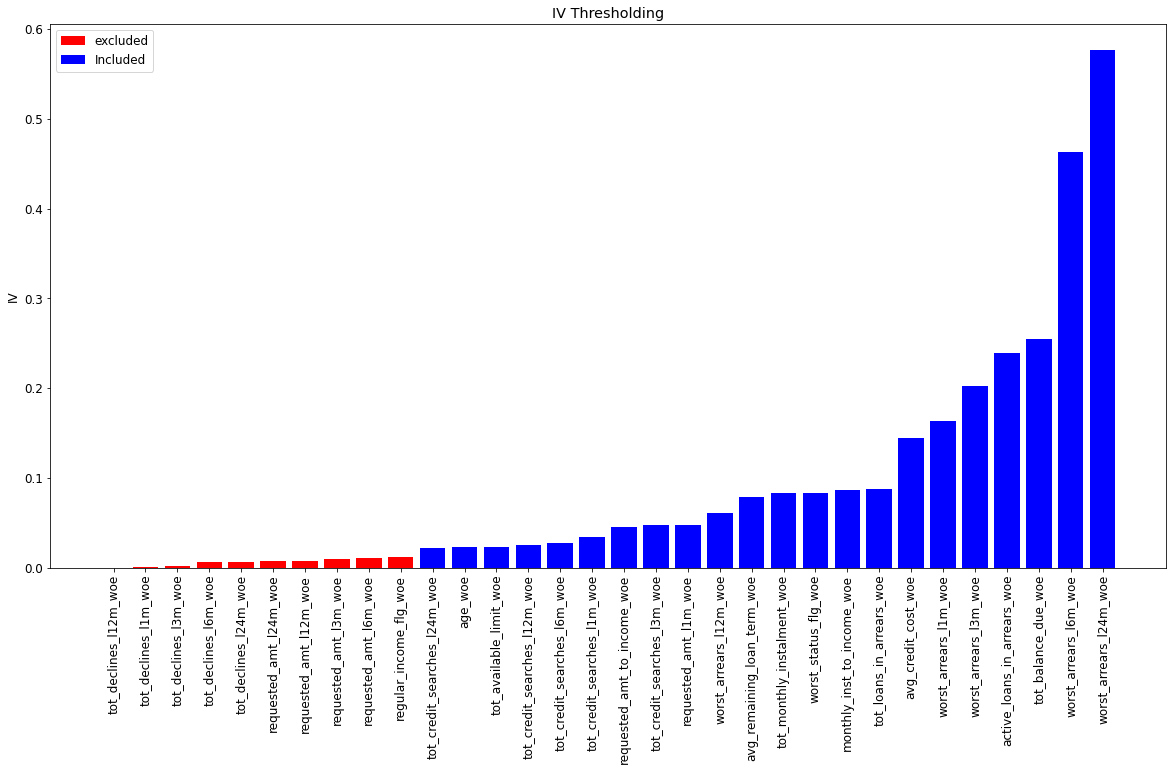
\includegraphics[width=\linewidth]{Credit_Images/IV.png}
   \caption{Information Value Thresholding.}
    \label{fig-IV-Thresh}
\end{figure}

\subsubsection{L1 Regularizer} For our raw features we use a model trained with a L1 regularizer which is referred to as a \emph{Lasso} model for feature selection. L1 regularization is able to assign higher weighting to features which play a larger role in classification and in turn can set those that do the least to 0. 
Given a linear model,
\begin{equation}
Y = \beta_{1}x_{1} + \beta_{2}x_{2} + ... + \beta_{0},
\end{equation}
where $Y$ is the label, $x_{i}$ are the features and $\beta_{i}$ are the weight coefficients.
The cost function can be written as,
\begin{equation}
\sum_{i=1}^{m}(Y_{i} - \sum_{j=1}^{n} \beta_{j}x_{ij})^{2},
\end{equation}
where $m$ is all the input samples in the training set and $n$ is the number of features in a sample.
We add a regularization term with the L1 penalizer,
\begin{equation}
        \sum_{i=1}^{m}(Y_{i} - \sum_{j=1}^{n} \beta_{j}x_{ij})^{2} + \lambda \sum_{j=1}^{n} |\beta_{j}|,
\end{equation}
where $\lambda$ is a coefficient that we can tune to adjust how aggressively we constrain our weights. Figure \ref{fig-lasso} demonstrates the constraint region built by the L1 regularizer for a model which contains two weight coefficients $\beta_{1}$ and $\beta_{2}$. $\overset{\wedge}{\beta}$ is the unconstrained least squares estimate. The red ellipses are the contours of the least squares error function. The blue area represents the feasible region $|\beta_{1}| + |\beta_{2}| \leq t$ of the constraints introduced by our penalty where $t$ is the coefficient of our regularizer. The possible values are those where the contour and diamond meet and as we can see  at 4 points of the diamond one of the weight coefficients are 0. This extends to higher dimensions where the are more possibilities of weights being 0. We are looking for the intersection of the red ellipses and the blue region as the objective is to minimize the error function while maintaining the feasibility. Let $p$ be the number of features and therefore the dimensionality, in this case we have $p = 2$. When $p > 2$ the diamond becomes a rhomboid and has many corners flat edges and faces which have the opportunity to become 0.
\begin  {figure}[!htpb]
\centering
  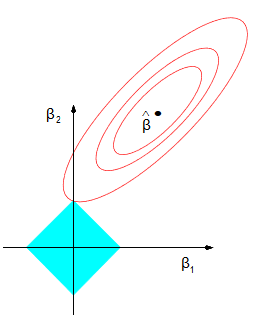
\includegraphics[width=0.5\linewidth]{Credit_Images/Lasso-regression.png}
   \caption{Boundary of lasso model.\cite{Hastie2009ThePrediction}}
    \label{fig-lasso}
\end{figure}

\subsubsection{Selecting our regularization coefficient}
As discussed in the previous section the higher we set the value of our regularization term the stricter we constrain our weight coefficients. Therefore the larger $\lambda$ is the stricter our feature selection is as more coefficients will be set to 0. In order to select a $\lambda$ that provides us with the best features we need to tune this as a hyper parameter by using our validation set. We need to make sure that we do not throw away any features that have information that cannot be explained by our selected features. Therefore we tune $\lambda$ by making it stricter and monitoring how it affects the performance of our model. In Figure \ref{fig-regularizer} we have plotted the results of the \emph{accuracy}, \emph{recall}, and \emph{precision} metrics against a stronger penalty. Note that the L1 coefficient in this case is inversely proportional to how strict our regularizer is. As we can see both the recall and precision takes quite a significant drop once $\lambda$ reaches $0.0001$. Therefore $0.001$ is the smallest that we can set $\lambda$ before we start noticing a drop in the performance of our model. Setting $\lambda$ to $0.001$ reduces our number of features from 33 to 17. This is a massive reduction while hardly losing any strength within our model, this may not be the most stable approach if we are looking to productionize this model but it allows our interpretation to be simpler to showcase due to the reduced number of attributions. These features are described in the \emph{Feature descriptions} section.
\begin  {figure}[!htpb]
\centering
  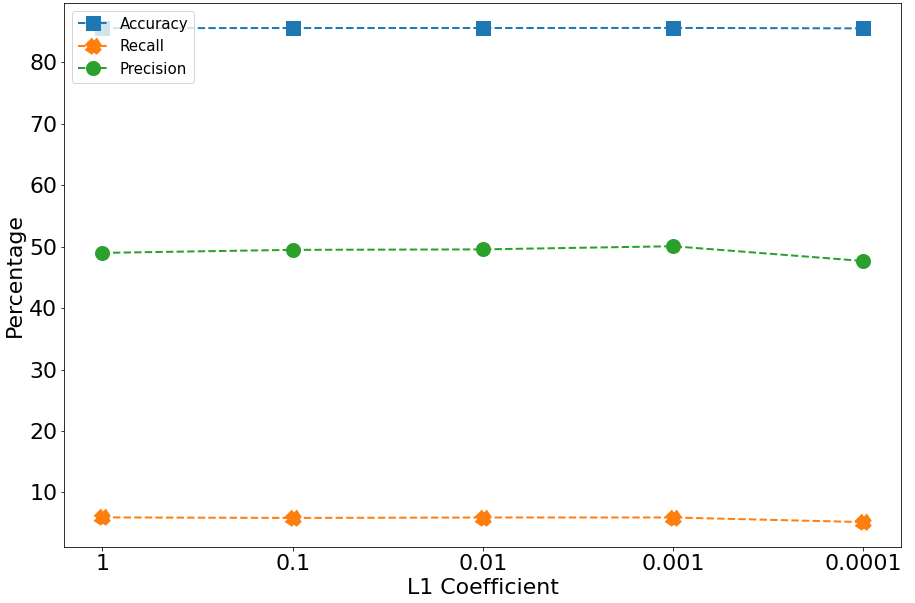
\includegraphics[width=\linewidth]{Credit_Images/Regularizer.png}
   \caption{Choosing our L1 coefficient.}
    \label{fig-regularizer}
\end{figure}

\subsection{Class imbalance} \label{sec-class-imbalance}
Class imbalance has a significant effect on conventional classification techniques because they assume a balance of classes \cite{articled}. In credit companies it is expected that there is a noticeable class imbalance within their data because they can not afford to have many bad loans \cite{809773}\cite{doi:10.1142/9789812813312_0009}. This results in there being far more loans which could be considered \emph{good}. This makes it difficult for many machine-learning techniques to learn the boundary between a good and bad loan because it does not have enough bad loans to properly identify them. Selectively sampling from the data in order to create a balanced dataset \cite{article} is a possible solution however this results in a far smaller training set and thus has an overall negative impact if we have a small sample size. It can be shown that by providing misclassification costs to our model provides an increase in the performance of classifiers  \cite{Vinciotti2003ScorecardCW}.  If we suppose that misclassifying a client that belongs to the \emph{default} as the \emph{not default} class is $r$ times as serious as the reverse. We can provide a weighting which penalize such misclassifications $r$ times as heavily as the reverse. In order to minimise the overall weighted misclassification rate we have to minimise,
\begin{equation}
  \mbox{ Assign to class} \ 1 \ \mbox{if} \ p(1|x) > (1 + r)^{-1} \mbox{and to class} \ 0 \ \mbox{otherwise}
\end{equation}
  We can incorporate these misclassification costs into our model by providing a weighting of classes which penalizes our model more for predicting the less present class incorrectly which is the \emph{default} class in our case. By using these bias class weights we may be able to identify more clients which may default, however we lose some accuracy in predicting non defaulting clients. 
\begin{equation}
    \mbox{Class weights} = \frac{|X|}{|y| \cdot \left[ y_{1}, ..., y_{n} \right]}
\end{equation}
Where $|X|$ is the number of samples, $|y|$ is the number of classes, $y_{i}$ is the number of labels of class $i$.
By using the values in our dataset we get,
\begin{flalign}
    \begin{split}
    \mbox{Class weights} &= \frac{120000}{2 \cdot \left[102739, 17261 \right]}
    \\
                         &= [0.584, 3.476]
    \end{split}
\end{flalign}
by using these class weights our model is penalized roughly $5.95$ times more for incorrectly classifying \emph{defaulting} clients as \emph{not defaulted}. This causes our weights to be optimized to predict the default class more. For our raw input models we will versions with and without these biased class weights and compare their results and how their interpretations differ.

\section{Models}
\subsection{Logistic Regression}
Logistic Regression is a widely used technique. Even some Deep Neural Networks use it within their output layer. It is known to work well for binary classification problems and provides a soft prediction. 
\subsubsection{Soft Predictions}
A soft prediction refers to a prediction which gives the probability that a input belongs to a specific class, where as a hard prediction simply assigns a 0 or 1 regardless if the prediction was on the boundary between the two classes. In Figure \ref{fig:thresholds} we can see difference between the thresholding mechanisms used in hard and soft predictions, the x-axes represents the output before  we threshold and the y-axes is the value that after it goes through our activation function. When using a hard threshold the values are either set to 0 or 1. For soft threshold the value is set as a probability between 0 and 1, this allows us see the confidence of our model in our prediction. For example in Figure \ref{fig:thresholds} if our value is 0, hard thresholding will force it to 1, however soft thresholding would set it to 0.5 which indicates that it could belong to either class. 

\subsubsection{Making a prediction using Logistic Regression}
Given a general linear model,
\begin{equation}
    y = \sum^{n}_{i = 1} w_{i} \cdot x_{i} + w_{0},
    \label{eq:linear}
\end{equation}
where $n$ is the number of features in our input.
We introduce the logistic function, or more commonly referred to as \emph{sigmoid}\cite{10.5555/1671238},
\begin{equation}
    \mbox{Sigmoid}(z) = \frac{1}{1 + e^{-z}}
\end{equation}
Substituting in (\ref{eq:linear}), this can be rewritten as,
\begin{equation}
    \mbox{Sigmoid}(w \cdot x + w_{0}) = \frac{1}{1 + e^{-(w \cdot x + w_{0})}}
    \label{eq:logistic}
\end{equation}
Once our model is trained, we substitute our input vector into (\ref{eq:logistic}) in order to make a prediction.
\begin{figure}
\centering
\begin{subFigure}{.5\textwidth}
  \centering
  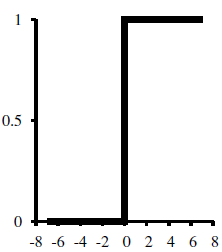
\includegraphics[width=\linewidth]{Credit_Images/hard_threshold.png}
  \caption{Hard Threshold}
  \label{fig:hard-threshold}
\end{subFigure}%
\begin{subFigure}{.5\textwidth}
  \centering
  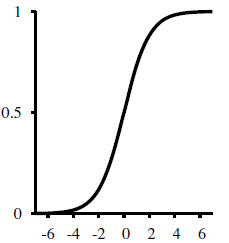
\includegraphics[width=\linewidth]{Credit_Images/soft_threshold.png}
  \caption{Soft Threshold}
  \label{fig:soft-threshold}
\end{subFigure}
\caption{Comparison of hard and soft thresholds\cite{10.5555/1671238}.}
\label{fig:thresholds}
\end{figure}
\subsubsection{Cross entropy cost function}
The cost function is a measure of how wrong the model is in terms of its ability to estimate the relationship between X and y. It can also be seen as the distance between our predicted labels and the actual labels.
Let our the sigmoid function of our model be $h_{w}(x)$ and our cost function be $J(w)$ then,
\abovedisplayskip=0pt\relax
\[
J(w) =
\begin{cases}
-\log(h_{w}(x)) & \text{if } y=1\\
-\log(1 - h_{w}(x)) & \text{if } y=0
\end{cases}
\]
can be condensed as,
\begin{equation}
J(w) = - \frac{1}{m} \sum_{i=1}^{m} \left[ y^{(i)}log(h_{w}(x^{(i)})) + (1 - y^{(i)})log(1-h_{w}(x^{(i)}))\right]
\end{equation}
Now that we have our cost function, we need to somehow decrease it until our weights converge.

\subsubsection{Gradient Descent}
In order to find the optimal parameters for our weights we have to minimize our cost function using gradient descent. Let $y$ be the true labels and $h_{w}(x)$ be our predicted labels. When using gradient descent, we set our weights to some initial value either randomly or by some initialization algorithm. We can update our weights by subtracting the derivative of the cost function,

\begin{equation}
w_{j} \longleftarrow w_{j} - \alpha \cdot \nabla_{w}J(w)
\end{equation}
where $\alpha$ is referred to as the \emph{learning rate} which is how large the steps we take when updating our weights. Since $h_{w}$ is the sigmoid function we can simplify this to, 
\begin{equation}
    w_{j} \longleftarrow w_{j} - \alpha \sum_{i=1}^{m}(h_{w}(x^{(i)}) - y^{(i)})x_{j}^{(i)}
\end{equation}
This continues until our weights have converged.
In Figure \ref{fig-gradient-descent} we can how our weights update during gradient descent. We start at some initial weights and after each weight update iteration we try to reach the minimum of our cost function. When we reach we the minimum our weights are considered to have converged and our training as completed as we have found our optimal parameters. Note that most if not all of the popular optimization procedures in Neural Networks is based on this simple idea, because the gradient can be efficiently calculated using \emph{back-propagation}. It should also be noted that numerous important modifications have been made for the sake of efficiency and robustness.
\begin {figure}[!htpb]
\centering
  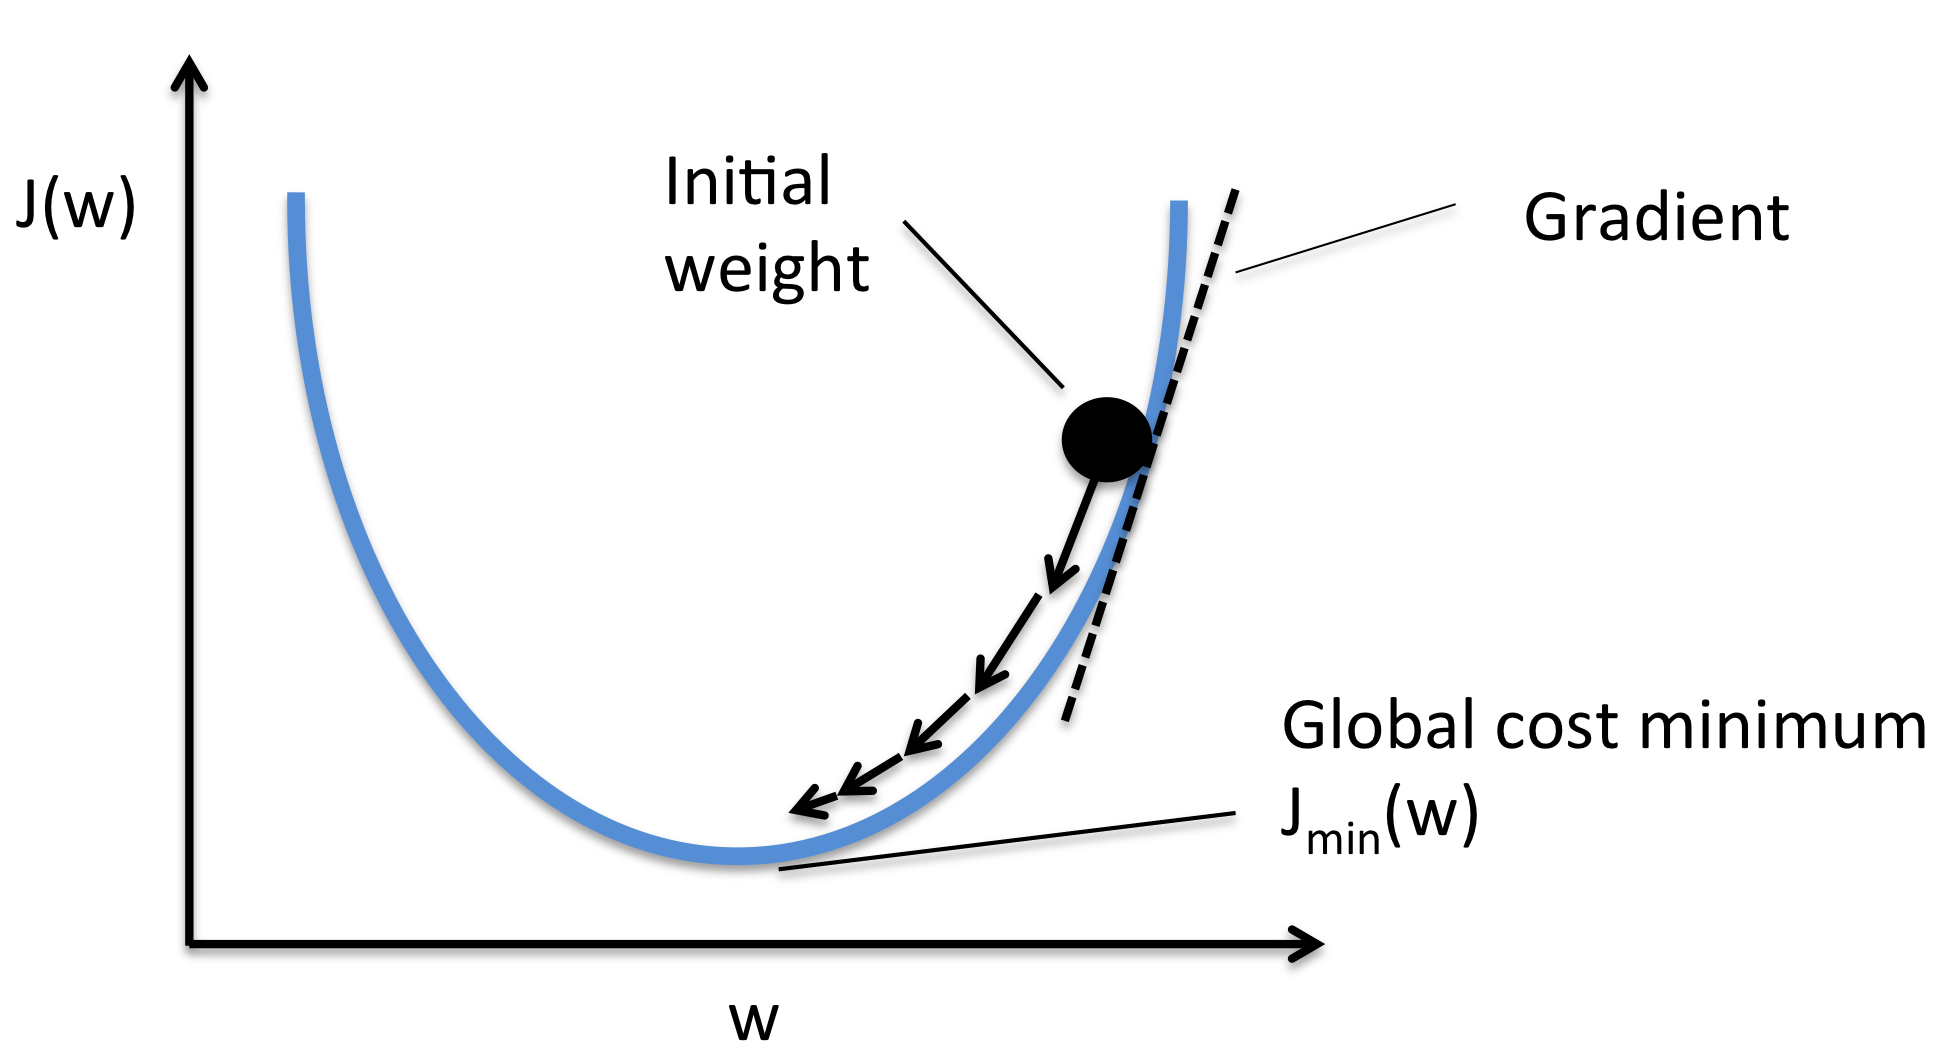
\includegraphics[width=\linewidth]{Credit_Images/GradientDescent.png}
   \caption{Gradient Descent \cite{GradientDescent}}
    \label{fig-gradient-descent}
\end{figure}

\subsubsection{Interpreting Logistic Regression} \label{sect:interpreting-logistic-regression}
Since the outcome of Logistic Regression is a probability between 0 and 1, we can not simply look at the weight coefficients as a direct interpretation. Due to the weighted sum being transformed by the sigmoid function (\ref{eq:logistic}) into a probability the weights do not influence the probability linearly. Introducing the log odds function,

\begin{equation}
    \log \left( \frac{P(y=1)}{1 - P(y=1)} \right) - \log \left( \frac{P(y=1)}{P(y=0)} \right) = w_{0} + w_{1}x_{1} + ... + w_{n}x_{n}
\end{equation}
We can adjust this equation in order to determine how the prediction changes when one feature $x_{j}$ is changed by 1 unit \cite{molnar2019}. Applying the exp function to both sides we end up with,

\begin{equation}
     \frac{P(y=1)}{1 - P(y=1)} = odds = \exp( w_{0} + w_{1}x_{1} + ... + w_{n}x_{n})
\end{equation}
Comparing the ratio of two predictions when increasing a single feature by 1,

\begin{equation}
    \frac{odds_{x_{j}+1}}{odds} = \frac{\exp^( w_{0} + w_{1}x_{1} + ... + w_{j}(x_{j} + 1) + ... w_{n}x_{n})}{exp^( w_{0} + w_{1}x_{1} + ... + w_{j}x_{j} + ... w_{n}x_{n})}
\end{equation}
Then applying the following exponential rule,

\begin{equation}
    \frac{\exp(a)}{\exp(b)} = \exp(a - b)
\end{equation}
and removing many terms,

\begin{equation}
    \frac{odds_{x_{j}+1}}{odds} = \exp(w_{j}(x_{j} + 1) - w_{j}x_{j}) = \exp(w_{j})
    \label{eq-odds-ratio}
\end{equation}
The \emph{Odds Ratio (OR)} is a measure of association between exposure and an outcome. The OR represents the odds that an outcome will occur given a particular exposure, compared to the odds of the outcome occurring in the absence of that exposure \cite {Szumilas2010ExplainingRatios}.
\begin{itemize}
    \item OR=$1$ Exposure does not affect odds of outcome
    \item OR$>1$ Exposure associated with higher odds of outcome
    \item OR$<1$ Exposure associated with lower odds of outcome
\end{itemize}
Therefore according to according to (\ref{eq-odds-ratio}) a change in a feature by one unit changes the odds ratio (multiplicative) by a factor of $\exp(w_{j})$. Another interpretation is that by changing a feature's value by one unit increases the log odds ratio by the value of the corresponding weight \cite{molnar2019}. Interpretation is different depending on the feature type \cite{molnar2019}:
\begin{itemize}
    \item \emph{Numerical features}: If you increase the value of feature $x_{j}$ by one unit, the estimated odds change by a factor of $\exp(w_{j})$
    \item \emph{Binary categorical features}: We refer to one of the categories as the \emph{reference} category. Changing the feature $x_{j}$ from the reference category to the other category in turn changes the estimated odds by a factor of $\exp(w_{j}))$.
    \item \emph{Categorical feature with more than two categories}:  When dealing with multiple categories one-hot-encoding is commonly used. For a feature which as N categories we would need N-1 columns in our one-hot-encoder. The N-th category is  considered the reference category.The interpretation for each category then is equivalent to the interpretation of binary features.
\end{itemize}
In table \ref{table:logistic} we can see an example of a Logistic Regression classifier trained to predict the probability of cervical cancer given certain risk factors. Looking at the \emph{Num. of diagnosed STDs} feature which is numerical increasing the number of STDs by 1 would in turn increase the odds of cancer vs. no Cancer by a factor of 2.26. Looking at the feature \emph{Hormonal contraceptives y/n} which is a binary categorical feature indicates that for women who use hormonal contraceptives, the odds for cancer vs. no cancer are by a factor of 0.89 lower, compared to women without hormonal contraceptive. It is important to note that these interpretations are only true if every other feature stays the same.
 \begin{table}[h!]
 \footnotesize
\begin{center}
\shadowbox{\begin{minipage}[t]{0.75\columnwidth}%
    \begin{tabular}{l|c|c|c}
         & \textbf{Weight} & \textbf{Odds ratio} & \textbf{Std. Error}\\
            \hline
         Intercept & $-2.91$ & $0.05$ & $0.32$ \\
         Hormonal contraceptives y/n & $-0.12$ & $0.89$ & $0.30$ \\
         Smokes y/n & $\phantom{-}0.26$ & $1.29$ & $0.37$ \\
         Num. of pregnancies & $\phantom{-}0.04$ & $1.04$ & $0.10$ \\
         Num. of diagnosed STDs & $\phantom{-}0.82$ & $2.26$ & $0.33$ \\
         Intrauterine device y/n & $\phantom{-}0.62$ & $1.85$ & $0.40$ \\
    \end{tabular}
    \end{minipage}}
\par\end{center}
\caption{The results of fitting a logistic regression model on the cervical cancer dataset. Shown are the features used in the model, their estimated weights and corresponding odds ratios, and the standard errors of the estimated weights. \cite{molnar2019}}\label{table:logistic}
\end{table}

\subsection{Feedforward Neural Network}
We will be training a generic feedforward Neural Network with a single hidden layer. The architecture can be seen in Figure \ref{fig-ff-nn}. Every layer in our Neural Network is \emph{Fully Connected} which means that every incoming node is connected to every outgoing node. The input layer is simply our input features. Our \emph{hidden layer} contains $9$ nodes for our raw features and $11$ nodes for our WOE network. For both networks our output layer is a single node that uses the \emph{sigmoid} activation function which is the probability that the client will default. Our Neural Network only has a single hidden layer and is considered very small when compared to modern networks.

\begin  {figure}[!htpb]
\centering
  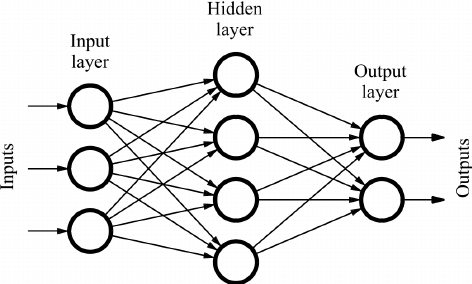
\includegraphics[width=0.9\linewidth]{Credit_Images/Sample-of-a-feed-forward-neural-network.png}
   \caption{Architecture of a generic Feedforward Neural Network \cite{inbook}.}
    \label{fig-ff-nn}
\end{figure}

\subsection{Trainable weights}
In order to show that a Neural Network is theoretically more powerful than Logistic Regression, we have to compare their \emph{trainable weights}. Trainable weights are the weights which our models will estimate in order to make a prediction. Theoretically the more weights we can estimate, the more accurate our predictions will be. However it is important that we account for \emph{overfitting} which is when our model corresponds too closely to our training data and thus fails to predict unseen data reliably. In practice there are other factors such as our networks architecture and preprocessing techniques which have an effect. We can calculate the trainable weights in our with,

\begin{equation*}
\begin{split}
    \mbox{LR} &= \mbox{Input weights} + \mbox{Intercept}
    \\
    \mbox{NN} &= \mbox{Input weights} \cdot \mbox{Hidden weights} + \mbox{Hidden weights} \cdot \mbox{Output weights}
    \end{split}
\end{equation*}
We can see the comparison of the trainable weights between our models in Figure \ref{table:trainable}.
 \begin{table}[h!]
 \footnotesize
\begin{center}
\shadowbox{\begin{minipage}[t]{\columnwidth}%
    \begin{tabular}{lccccc}
       \textbf{Model}  & \textbf{Input} & \textbf{Hidden} & \textbf{Output} & \textbf{Intercept} & \textbf{Trainable Weights}\\
        Logistic Regression & $17$ & 0 & 1 & $\checkmark$ &  18\\
        Logistic Regression WOE & $22$ & 0 & 1 & $\checkmark$ & 23\\
        Neural Network & $17$ & 9 & 1 & $\times$ & 162\\
        Neural Network WOE & $22$ & 11 & 1 & $\times$ & 253\\
    \end{tabular}
    \end{minipage}}
\par\end{center}
\caption{Trainable Weights}\label{table:trainable}
\end{table}
%%%% RESULTS %%%%
\section{Results}
In this section we will compare the following models:
\begin{itemize}
    \item Logistic Regression with raw inputs.
    \item Logistic regression with raw inputs and altered class weights.
    \item Logistic Regression with WOE inputs.
    \item Neural Network with raw inputs.
    \item Neural Network with raw inputs and altered class weights.
    \item Neural Network with WOE inputs.
\end{itemize}

\begin {figure}[!htpb]
\centering
  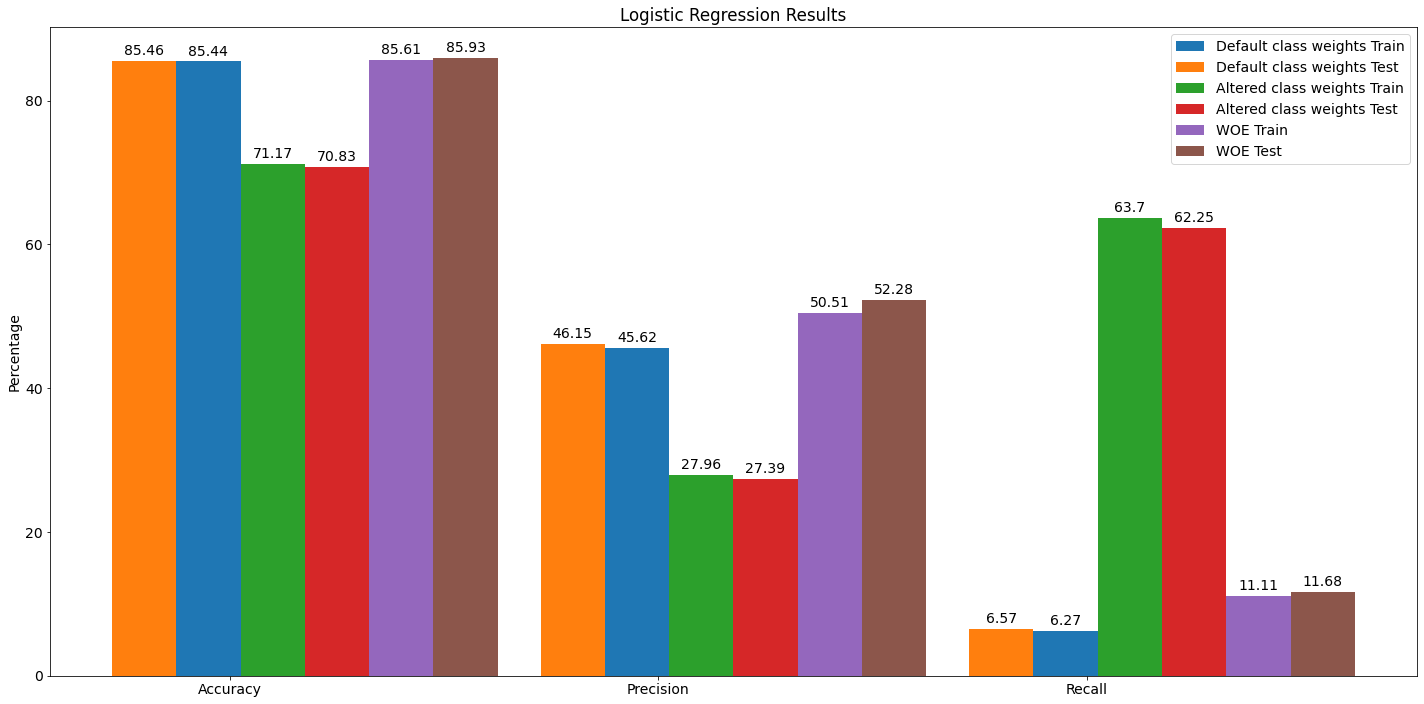
\includegraphics[width=\linewidth]{Credit_Images/Results_Logistic.png}
   \caption{Results of our Logistic Regression classifier.}
    \label{fig-log-results}
\end{figure}
\begin {figure}[!htpb]
\centering
  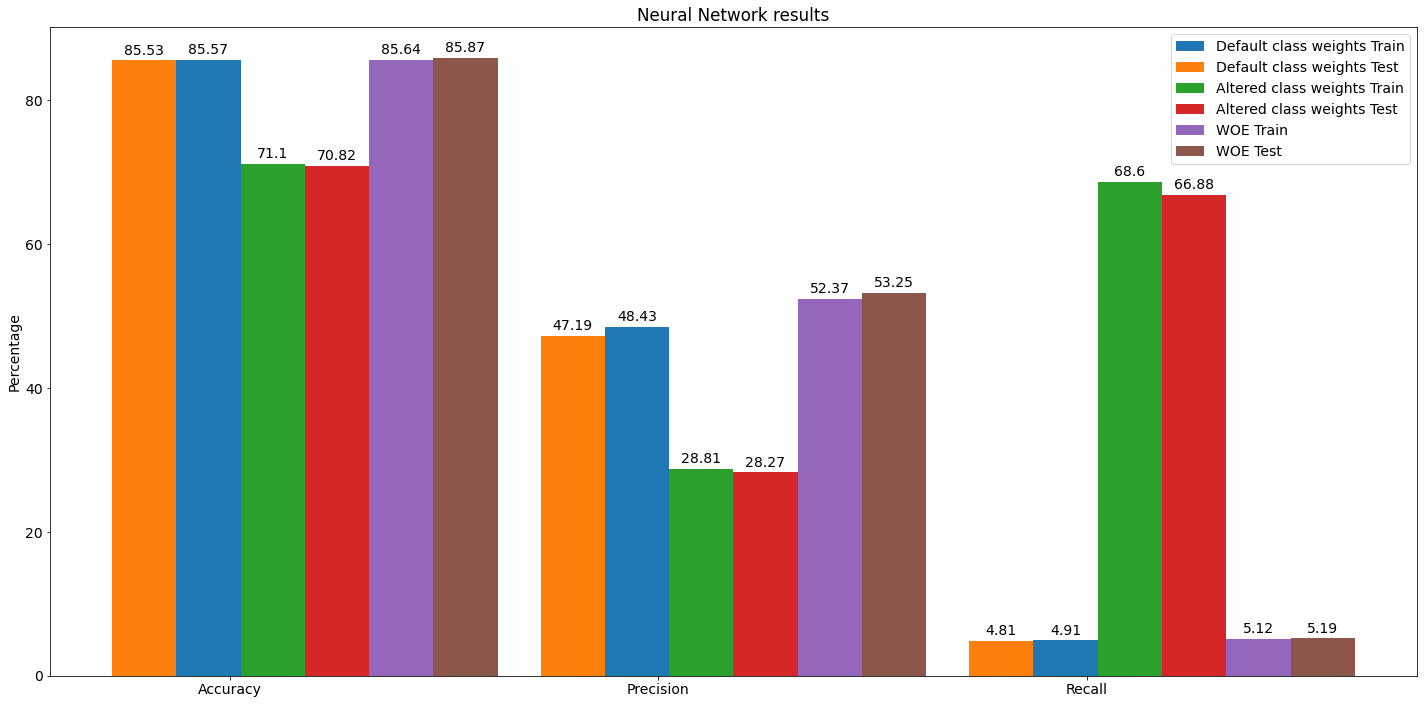
\includegraphics[width=\linewidth]{Credit_Images/NN_res.png}
   \caption{Results of our Neural Network.}
    \label{fig-nn-results}
\end{figure}

\subsection{Comparison}
Comparing the results from our Logistic Regression classifier in Figure \ref{fig-log-results} and Neural Network classifier in Figure \ref{fig-nn-results} their \emph{accuracy} is mostly the same with the only real difference being a slight increase in \emph{precision} and \emph{recall} in our Neural Network. From this it may seem that there is no reason to use a Neural Network classifier, however there are plenty of optimizations and various other network compositions that may provide better results. Our purpose is to provide interpretability and therefore we are not concerned with building the most robust network possible.
\subsection{Normal vs Bias class weights}
In both models when using the bias class weights discussed in the \emph{Class imbalance} section we see on average a $15\%$ drop in accuracy which is quite significant, however an enormous increase in \emph{recall} which means the bias versions are better at identifying clients which \emph{defaulted}. For credit companies where the purpose is to identify clients which may default on their loans, the bias weights provide better results. In the upcoming \emph{Interpretation} section we compare both the normal and bias class weights models and observe the explanations produced by SHAP in order to compare the difference in feature attributions. 
\subsection{Raw Inputs vs WOE}
When looking at the comparisons from the raw input features to the WOE transformed features in both our Logistic Regression results in Figure \ref{fig-log-results} and our Neural Network results in Figure \ref{fig-nn-results} there does not some to be a significant difference. The only noticeable difference is a slight increase in precision. WOE transformation are the standard when working in the credit industry and from these results it may seem like there isn't much merit in it, but we will see in our \emph{explanations} in section \ref{sec-interpretation} that there is a significant difference.
 \section{Feature descriptions} \label{sect-Feature-Descriptions}
 In order to make sense of feature attribution we first have to describe what each feature means. From our credit domain knowledge we are able to specify which features magnitudes increase proportionally to the risk that the client will default.
 
 \subsection{Not Default}
 The following features decrease the risk of the client defaulting,
 \begin{description}
     \item[age (For clients who are middle-aged)] \hfill \\ The age of the client.
     \item[regular\_income\_flg] \hfill \\ A flag which indicates whether the client has a regular income or not.
     \item[tot\_available\_limit] \hfill \\ Total monthly limit available to client.
 \end{description}
 \subsection{Default}
 The following features increase the risk of the client defaulting,
 \begin{description}
     \item[age (For clients who are very young or old)] \hfill \\ The age of the client.
     \item[requested\_amt\_l1m] \hfill \\ Requested amount over a month.
     \item[requested\_amt\_l24m] \hfill \\ Requested amount over 24 months.
     \item[requested\_amt\_to\_income] \hfill \\ Ratio of requested amount to monthly income.
     \item[avg\_credit\_cost] \hfill \\ Average cost of credit.
     \item[avg\_remaining\_loan\_term] \hfill \\ The average amount of months left on the clients loans.
     \item[tot\_monthly\_instalment] \hfill \\ Monthly installment paid towards the loan.
     \item[monthly\_inst\_to\_income] \hfill \\ Ratio of income to monthly installment.
     \item[tot\_credit\_searches\_l1m] \hfill \\ Total credit searches in the last month.
     \item[tot\_credit\_searches\_l3m] \hfill \\ Total credit searches in the last 3 months.
     \item[tot\_credit\_searches\_l6m] \hfill \\ Total credit searches in the last 6 months.
     \item[tot\_credit\_searches\_l12m] \hfill \\ Total credit searches in the last 12 months.
     \item[tot\_credit\_searches\_l24m] \hfill \\ Total credit searches in the last 24 months.
     \item[worst\_status\_flg] \hfill \\ Flag of whether this loan is the most in arrears.
     \item[tot\_declines\_l12m] \hfill \\ Total credit declines in the last 12 months.
     \item[active\_loans\_in\_arrears] \hfill \\ Active loans that are in arrears.
     \item[tot\_loans\_in\_arrears] \hfill \\ Total loans that are in arrears.
     \item[worst\_arrears\_l1m] \hfill \\ Worst arrears in the past month.
     \item[worst\_arrears\_l3m] \hfill \\ Worst arrears in the past 3 months.
     \item[worst\_arrears\_l6m] \hfill \\ Worst arrears in the past 6 months.
     \item[worst\_arrears\_l12m] \hfill \\ Worst arrears in the past 12 months.
     \item[worst\_arrears\_l24m] \hfill \\ Worst arrears in the past 24 months.
     \item[tot\_balance\_due] \hfill \\ Total balance due on the loan.
 \end{description}
%%%% Interpretation %%%%
\section{Interpretation} \label{sec-interpretation}
In this section we observe how the inherent interpretability of Logistic Regression compares to the explanations provided by SHAP of our Neural Network. We provide interpretation for both the normal and bias class weights models as well as a comparison between the attributions generated by our WOE features compared to the raw features.
\subsection{Logistic Regression}
As we have discussed in section \ref{sect:interpreting-logistic-regression} for Logistic Regression the weight coefficients are not enough to provide interpretability.  We have to extract the weight coefficients $w$ from the linear equation (\ref{eq:linear}) and also calculate their odds ratio (which is described in section \ref{sect:interpreting-logistic-regression}) with (\ref{eq-odds-ratio}). We have tabulated the weight coefficients as well as their respective odds ratios. We have also graphed the odds ratio for extra clarity. Table \ref{table:logistic} and Figure \ref{fig-odds-lr}  is for our raw input model. Table \ref{table:logistic-weighted} and Figure \ref{fig-odds-weighted} is for our raw input model with altered class weights. Lastly table \ref{table:logistic-woe} and Figure \ref{fig-odds-woe} is for our WOE model.

\subsubsection{WOE weight coefficients}
From table \ref{table:logistic-woe} we can see that all of our weight coefficients are positive for our WOE classifier. It may seem like every variable positively contributes towards the \emph{default} class. This is however not the case as we do not know the range of the magnitudes of our variables by just looking at this table. If the woe value of a feature in a specific bin is negative then even if the weight coefficient is positive it will provide a negative attribution. Therefore table \ref{table:logistic-woe} can not be considered sufficient information as we would need to view the range of the feature values to discern whether a feature decreases or increases the probability of \emph{defaulting}.

 \begin{table}[h!]
 \footnotesize
\begin{center}
\shadowbox{\begin{minipage}[t]{0.55\columnwidth}%
    \begin{tabular}{l|c|c}
         \textbf{Feature} & \textbf{Weight} & \textbf{Odds ratio}\\
            \hline
         requested\_amt\_l24m & $\phantom{-}0.0028$ & $1.002804$ \\
         tot\_declines\_l12m & $\phantom{-}0.0098$ & $1.009848$ \\
         requested\_amt\_to\_income & $\phantom{-}0.0109$ & $1.010960$  \\
         tot\_credit\_searches\_l12m & $-0.0207$ & $0.979513$  \\
         worst\_arrears\_l24m & $\phantom{-}0.0233$ & $1.023574$  \\
         tot\_available\_limit & $-0.0305$ & $0.969960$  \\
         tot\_credit\_searches\_l3m & $\phantom{-}0.0335$ & $1.034067$  \\
         age & $-0.0474$ & $0.953706$ \\
         tot\_loans\_in\_arrears & $\phantom{-}0.0565$ & $1.058127$ \\
         regular\_income\_flg & $-0.0645$ & $0.937536$ \\
         tot\_monthly\_installment & $-0.0659$ & $0.936224$ \\
         worst\_status\_flg & $\phantom{-}0.0676$ & $1.069937$ \\
         avg\_credit\_cost & $\phantom{-}0.0781$ & $1.081231$  \\
         monthly\_inst\_to\_income & $\phantom{-}0.0832$ & $1.086759$  \\
         avg\_remaining\_loan\_term & $\phantom{-}0.0846$ & $1.088282$  \\
         worst\_arrears\_l6m & $\phantom{-}0.1027$ & $1.108159$  \\
         active\_loans\_in\_arrears & $-0.2181$ & $0.804045$  \\

    \end{tabular}
    \end{minipage}}
\par\end{center}
\caption{Weight coefficients for Logistic Regression}\label{table:logistic}
\end{table}

\begin  {figure}[!htpb]
\centering
  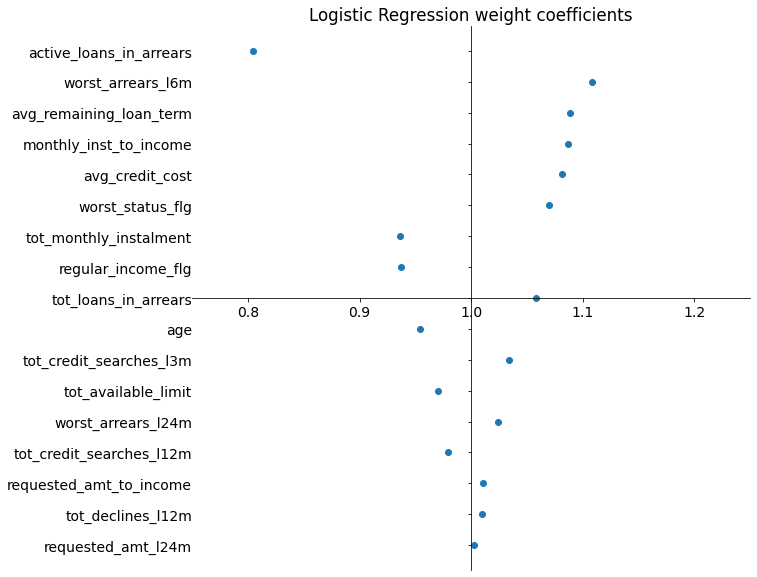
\includegraphics[width=0.8\linewidth]{Credit_Images/LR_ODDS.png}
   \caption{Odds ratios for Logistic Regression}
    \label{fig-odds-lr}
\end{figure}


 \begin{table}[h!]
 \footnotesize
\begin{center}
\shadowbox{\begin{minipage}[t]{0.55\columnwidth}%
    \begin{tabular}{l|c|c}
         \textbf{Feature} & \textbf{Weight} & \textbf{Odds ratio}\\
            \hline
         requested\_amt\_l24m & $-0.0076$ & $0.992429$  \\
         tot\_declines\_l12m & $\phantom{-}0.0497$ & $1.050956$ \\
         requested\_amt\_to\_income & $\phantom{-}0.0161$ & $1.016230$   \\
         tot\_credit\_searches\_l12m & $-0.0172$ & $0.982947$  \\
         worst\_arrears\_l24m & $\phantom{-}0.0769$ & $1.079934$   \\
         tot\_available\_limit &  $\phantom{-}0.0171$ & $1.017247$ \\
         tot\_credit\_searches\_l3m & $\phantom{-}0.0539$ & $1.055379$  \\
         age & $-0.0375$ & $0.963194$   \\
         tot\_loans\_in\_arrears & $\phantom{-}0.0339$ & $1.034481$  \\
         regular\_income\_flg & $-0.0481$ & $0.953038$ \\
         tot\_monthly\_installment & $-0.0819$ & $0.921364$ \\
         worst\_status\_flg & $\phantom{-}0.0475$ & $1.048646$  \\
         avg\_credit\_cost & $\phantom{-}0.0941$ & $1.098670$   \\
         monthly\_inst\_to\_income & $\phantom{-}0.0989$ & $1.103956$   \\
         avg\_remaining\_loan\_term & $\phantom{-}0.0609$ & $1.062793$   \\
         worst\_arrears\_l6m & $\phantom{-}0.0773$ & $1.080366$  \\
         active\_loans\_in\_arrears & $-0.1814$ & $0.834102$  \\

    \end{tabular}
    \end{minipage}}
\par\end{center}
\caption{Weight coefficients for Logistic Regression with altered class weights.}\label{table:logistic-weighted}
\end{table}

\begin  {figure}[!htpb]
\centering
  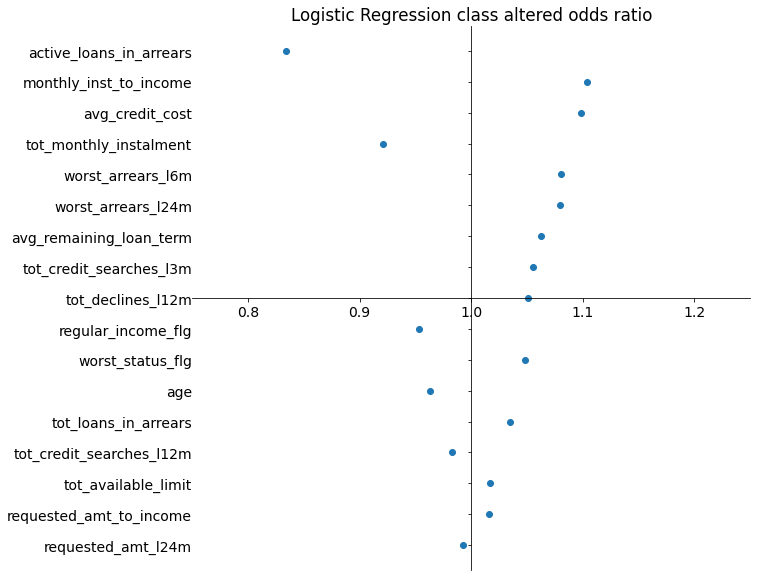
\includegraphics[width=0.8\linewidth]{Credit_Images/LR__ALTERED_ODDS.png}
   \caption{Odds ratios for Logistic Regression with altered class weights.}
    \label{fig-odds-weighted}
\end{figure}




 \begin{table}[h!]
 \footnotesize
\begin{center}
\shadowbox{\begin{minipage}[t]{0.6\columnwidth}%
    \begin{tabular}{l|c|c}
         \textbf{Feature} & \textbf{Weight} & \textbf{Odds ratio}\\
            \hline
            tot\_monthly\_instalment\_woe & $1.001401$ & $0.0014$ \\
            worst\_arrears\_l1m\_woe & $1.002102$ & $0.0021$ \\
            tot\_credit\_searches\_l6m\_woe & $1.004108$ & $0.0041$ \\
            worst\_arrears\_l3m\_woe & $1.009041$ & $0.0090$ \\
            worst\_status\_flg\_woe & $1.010859$ & $0.0108$ \\
            worst\_arrears\_l12m\_woe & $1.012984$ & $0.0129$ \\
            tot\_credit\_searches\_l24m\_woe & $1.015621$ & $0.0155$ \\
            tot\_credit\_searches\_l12m\_woe & $1.016332$ & $0.0162$ \\
            tot\_credit\_searches\_l1m\_woe & $1.017145$ & $0.0170$ \\
            requested\_amt\_to\_income\_woe & $1.024188$ & $0.0239$ \\
            worst\_arrears\_l6m\_woe & $1.040603$ & $0.0398$ \\
            tot\_credit\_searches\_l3m\_woe & $1.053376$ & $0.0520$ \\
            monthly\_inst\_to\_income\_woe & $1.056541$ & $0.0550$ \\
            tot\_loans\_in\_arrears\_woe & $1.057280$ & $0.0557$ \\
            avg\_credit\_cost\_woe & $1.059079$ & $0.0574$ \\
            tot\_balance\_due\_woe & $1.061412$ & $0.0596$ \\
            tot\_available\_limit\_woe & $1.064814$ & $0.0628$ \\
            requested\_amt\_l1m\_woe & $1.067159$ & $0.0650$ \\
            worst\_arrears\_l24m\_woe & $1.078100$ & $0.0752$ \\
            avg\_remaining\_loan\_term\_woe & $1.102963$ & $0.0980$ \\ 
            active\_loans\_in\_arrears\_woe & $1.109268$ & $0.1037$ \\
            age\_woe & $1.176919$ & $0.1629$

    \end{tabular}
    \end{minipage}}
\par\end{center}
\caption{Weight coefficients for WOE Logistic Regression.}\label{table:logistic-woe}
\end{table}

\begin  {figure}[!htpb]
\centering
  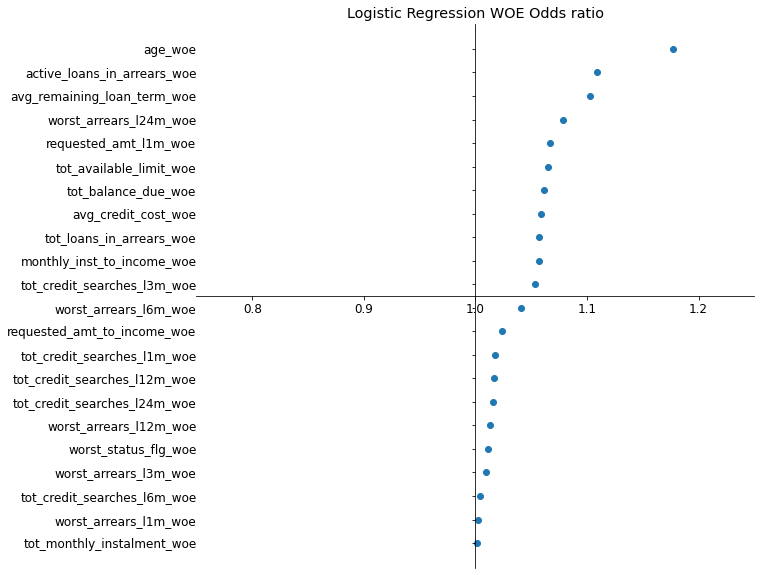
\includegraphics[width=0.8\linewidth]{Credit_Images/LR_WOE_ODDS.png}
   \caption{Odds ratios for WOE Logistic Regression.}
    \label{fig-odds-woe}
\end{figure}


\subsection{Neural Network}
For our Neural Network we will be using \emph{Deep SHAP} as it leverages the composition of Neural Networks to significantly increase the speed of SHAP.
We will be looking at how SHAP explains individual predictions as well as the explanation for the entire model.
\subsubsection{Model explanation}
We start by explaining on a global level the attributions our model assigns to each input feature and compare it to our Logistic Regression explanations. Figure~ \ref{fig-deep-shap-NN} is the explanation for our normal network, Figure \ref{fig-deep-shap-weighted-NN} is for our bias class weights network, and Figure \ref{fig-deep-shap-WOE-NN} is our WOE network. Rather than just giving a single value for attributions SHAP is able to plot over multiple instances in our dataset and showcase how each feature attributes to different instances. The y-axes are our feature names and the x-axes are their corresponding SHAP values, larger values impacts our model more. Positive values attribute towards the \emph{default} class and negative values to the \emph{not default} class. The hue of a point ranges from blue to red where the redder a point the larger the magnitude of that feature was in that particular instance.
\paragraph{Explanation}
Using the information from the \emph{Feature description} section we know that the larger the magnitude of the \emph{Age} feature the more it contributes against the client defaulting. In Figure \ref{fig-deep-shap-NN} and \ref{fig-deep-shap-weighted-NN} we can see that if the larger the magnitude of age the SHAP value falls more into the negative region, this indicates that the older the client is, the less likely they are to \emph{default}. This coincides with our knowledge. On the inverse we know that the \emph{avg\_credit\_cost} feature contributes towards the client default, this is also shown in Figure \ref{fig-deep-shap-NN} and \ref{fig-deep-shap-weighted-NN} where the instances where the magnitude of \emph{avg\_credit\_cost} is larger it's SHAP value and thus the higher contribution it had towards predicting that the client would default.

\begin  {figure}[!htpb]
\centering
  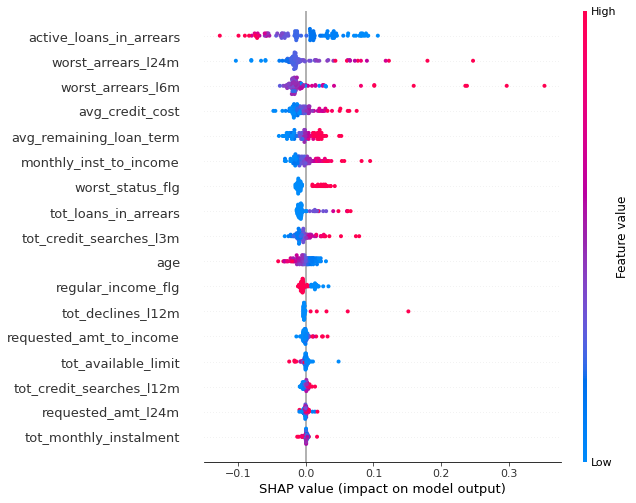
\includegraphics[width=0.8\linewidth]{Credit_Images/NN_shap_deep_summary.png}
   \caption{Deep SHAP interpretation for Neural Network.}
    \label{fig-deep-shap-NN}
\end{figure}

\begin  {figure}[!htpb]
\centering
  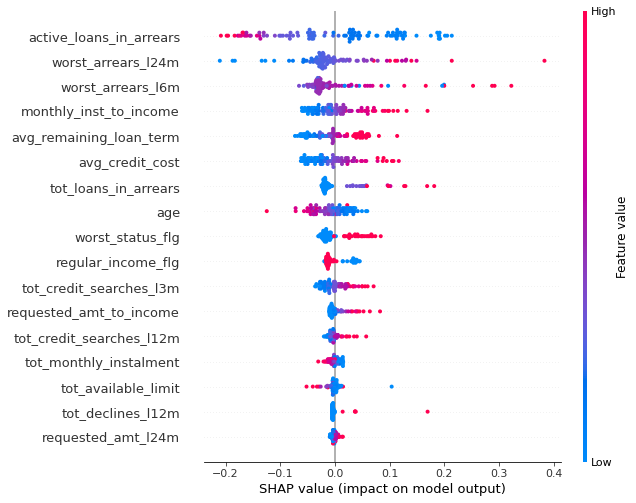
\includegraphics[width=0.8\linewidth]{Credit_Images/NN_shap_deep_weighted_summary.png}
   \caption{Deep SHAP interpretation for class weight bias Neural Network.}
    \label{fig-deep-shap-weighted-NN}
\end{figure}
\begin  {figure}[!htpb]
\centering
  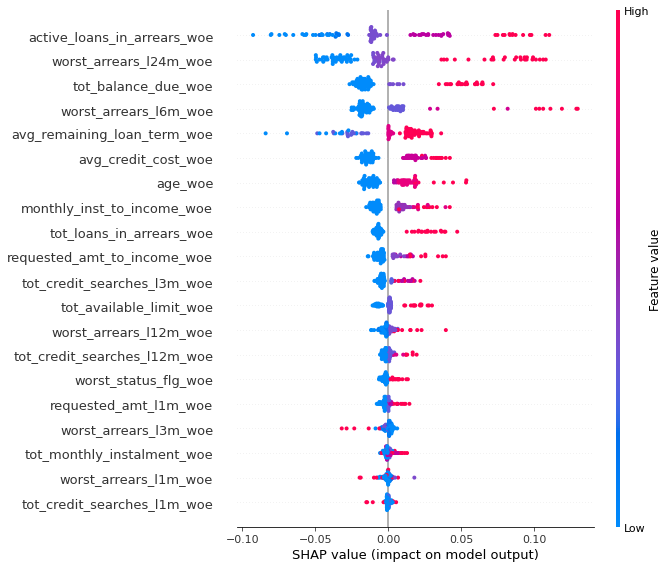
\includegraphics[width=0.8\linewidth]{Credit_Images/WOE_IV_NOSCALE_MODEL.png}
   \caption{Deep SHAP interpretation for WOE Neural Network.}
    \label{fig-deep-shap-WOE-NN}
\end{figure}

\subsubsection{Individual predictions}
An advantage of using a tool such as SHAP is that we are able to obtain explanations for individual predictions rather than just for the entire model. This is useful for credit employees as they this allows them to obtain explanations for an individual client. We have chosen a single client which has defaulted and in Figure \ref{fig-deep-shap-single-NN}, \ref{fig-deep-shap-weighted-single-NN} and \ref{fig-deep-shap-WOE-single-NN} we can see a plot of the explanation for it's prediction. Figure \ref{fig-deep-shap-single-NN} is the \emph{normal} class weights and the output of the model is that $27\%$ certain the client will \emph{default on their loan}. Figure \ref{fig-deep-shap-weighted-single-NN} is the explanation for the \emph{bias} class weights model and it is $71\%$ certain that the client will \emph{default}. Figure \ref{fig-deep-shap-WOE-single-NN} is the explanation for our WOE Neural Network and it is $37\%$ that the client will \emph{default}. The y-axes are the input features and the x-axes is the model output value. The bottom of the line is the average model output value, which the models default output value given that there is no information about the input features. As the line reaches the top, each feature either adds or subtracts from the models predicted value, therefore features that subtract from the value are negative attributions and those that add are positive attributions. The numbers in brackets are the values of that feature of this particular client standardized.

\begin  {figure}[!htpb]
\centering
  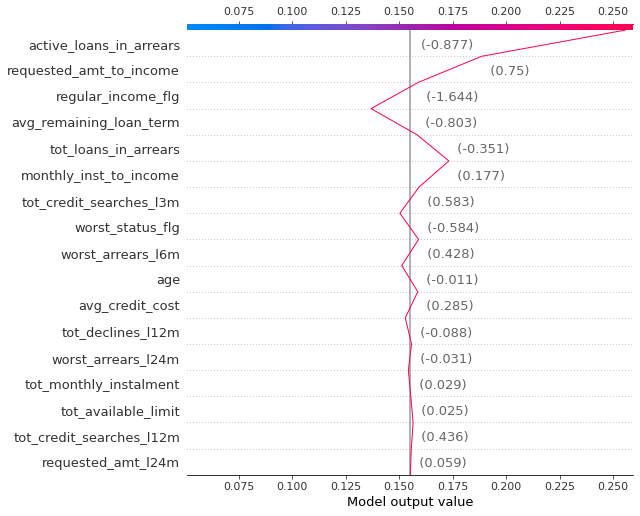
\includegraphics[width=0.8\linewidth]{Credit_Images/shap-nn-single.png}
   \caption{Single prediction Deep SHAP interpretation for Neural Network.}
    \label{fig-deep-shap-single-NN}
\end{figure}

\begin  {figure}[!htpb]
\centering
  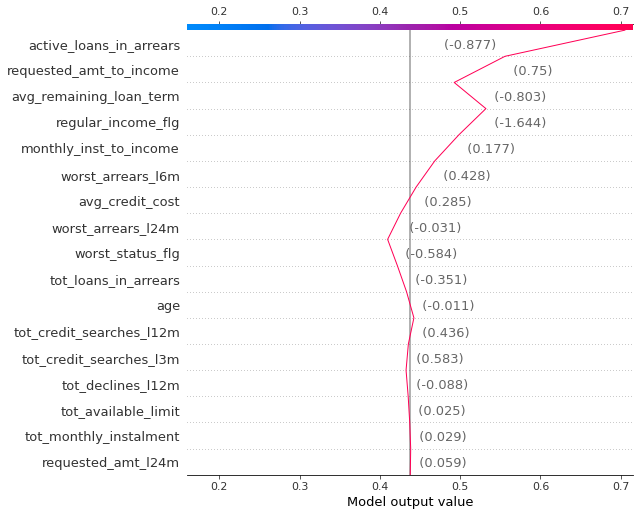
\includegraphics[width=0.8\linewidth]{Credit_Images/shap-nn-weighted-single.png}
   \caption{Single prediction Deep SHAP interpretation for class weight bias Neural Network.}
    \label{fig-deep-shap-weighted-single-NN}
\end{figure}

\begin  {figure}[!htpb]
\centering
  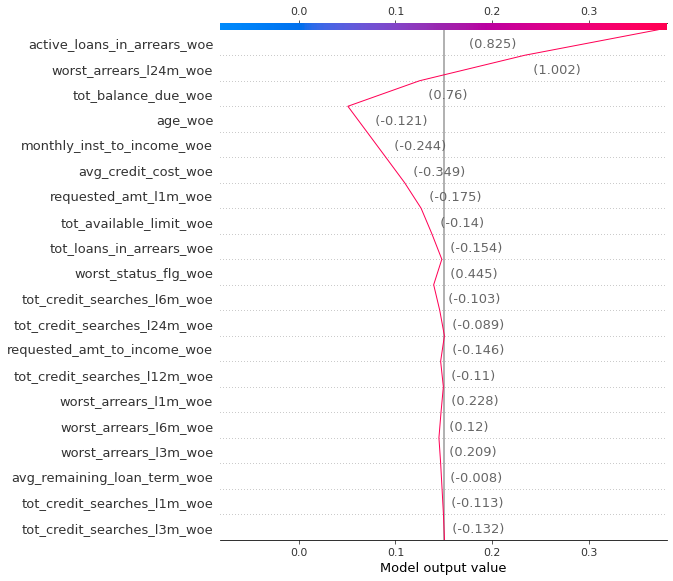
\includegraphics[width=0.8\linewidth]{Credit_Images/WOE_IV_NOSCALE_INDV.png}
   \caption{Single prediction Deep SHAP interpretation for WOE Neural Network.}
    \label{fig-deep-shap-WOE-single-NN}
\end{figure}


\subsection{Comparison} Comparing the weight coefficients obtained from Logistic Regression with the SHAP explanations we can see that although the SHAP values have a different meaning than the raw weight coefficients they are comparable. They both provide relative value of how much that particular feature would affect the prediction of our models. The SHAP explanations are far more descriptive as they are able to provide explanations over multiple instances, which shows consistency and we are also able to provide explanations for individual instances. Since the SHAP values are consistent with what we expect we can conclude that we have successfully provided explanations into this previously considered \emph{black-box} credit risk Neural Network.

\subsection{Exposing a problem with our raw input models} \label{sect-problem-expose}
If we refer back to section \ref{sect-Feature-Descriptions} we can see that  the \emph{active\_loans\_in\_arrears} feature is the number of active loans that the client currently has in arrears. An increase in its feature value would in turn cause the risk of the client to increase. As we can see for our WOE model in Figure \ref{fig-deep-shap-WOE-NN} the larger the magnitude of \emph{active\_loans\_in\_arrears} the higher the contribution towards the \emph{Default} class as expected. However looking at the SHAP explanations for our raw input models in Figure \ref{fig-deep-shap-NN} and \ref{fig-deep-shap-weighted-NN} the larger  \emph{active\_loans\_in\_arrears} is the less likely the client is to \emph{default} . This means that there is an obvious flaw present with our raw input models with regards to this feature. This is not obvious from just observing our Logistic Regression models since it hard to determine how the feature reacts over multiple instances and different magnitudes by only looking at the features overall contribution. Even though the performance of the two models are relatively the same by viewing the SHAP explanations produced , we were able to identify this problem.

\subsection{Monitoring changes within our architecture} \label{sect-architecure}
Figure \ref{fig-deep-shap-WOE-sig} is the SHAP explanation of our WOE Neural Network without the hidden layer. When comparing this to Figure \ref{fig-deep-shap-WOE-NN} there is a noticeable difference as the \emph{worst\_arrears\_l24m\_woe} has the largest contribution. Thus by using SHAP we are able to determine how a change in our networks architecture affects the feature attributions.
\begin{figure}[!htpb]
\centering
  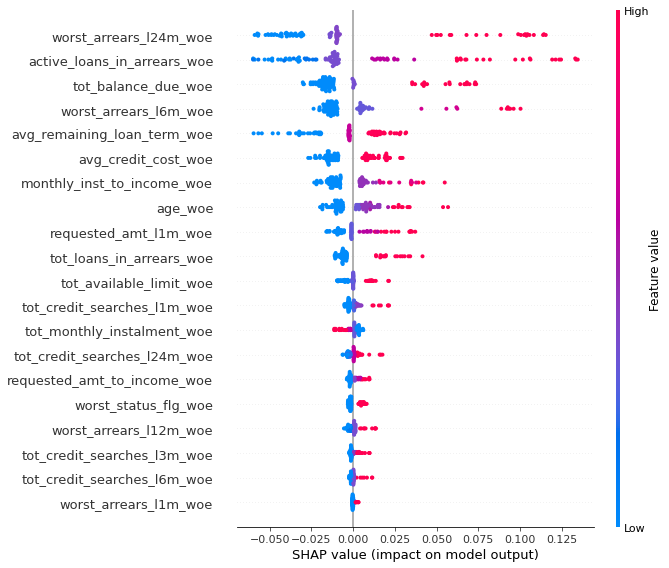
\includegraphics[width=0.8\linewidth]{Credit_Images/Sigmoid_nn_shap.png}
   \caption{Neural Network WOE with just the input layer and output sigmoid layer.}
    \label{fig-deep-shap-WOE-sig}
\end{figure}

\subsection{Attributions between normal and bias class weights}
Comparing the feature attributions between Figure \ref{fig-deep-shap-NN} and \ref{fig-deep-shap-weighted-NN}, there are a few key differences. The first is that the order of the features are different which means the features which contribute the most differ. Looking at \emph{monthly\_inst\_to\_income} and \emph{total\_loan\_in\_arrears} in Figure  \ref{fig-deep-shap-weighted-NN}, it can be seen that they have stronger attributions towards the \emph{default} class in our weighted model. Another notable difference is the \emph{worst\_arrears\_l24m\_feature}, in Figure \ref{fig-deep-shap-weighted-NN} the maximum value possible SHAP value is larger which means that this feature can have a larger effect on the models outcome. From this we can see that it seems that by using the misclassification costs introduced in section \ref{sec-class-imbalance} some of our features were given more predictive power towards the \emph{default} class.

\subsection{Prediction strength relative to Feature magnitude} \label{sect-prediction-strength}
With SHAP we are able to sample our explanations over multiple instances. If our chosen background instances are diverse, we are able to view how our feature attributions react over varying magnitudes. For example if we look at the odds ratio for \emph{worst\_status\_flg} in table \ref{table:logistic} we can see that the feature has an \emph{odds ratio} of $1.069937$ which by using our domain knowledge we know that this is a binary categorical variable which can only take on a value of 0 or 1. However if we did not have domain knowledge about this variable it could possibly be mistaken as a \emph{continuous variable} which makes it seem as though it could have a much larger contribution than it actually does. Now if we compare to this to our SHAP explanation in Figure \ref{fig-deep-shap-NN} we can see how the features contributions reacts at different values. From this we can see that regardless of it's magnitude the feature relatively has the same contribution if it is high and a small contribution when it is low. It would require more effort and observing the original feature to discern this from just the Logistic Regression explanation. This could possibly be used for \emph{Feature Selection}. By observing how the contribution of a feature changes over varying magnitudes we can choose to manually remove features which regardless of their intensity seem to add little value. If we once again look at Figure \ref{fig-deep-shap-NN}, the feature \emph{tot\_monthly\_instalment} seems have a very low SHAP Value even when it's feature value is high and could possibly be considered for removal. 